\subsection{Import ASTERIX Recording}
\label{sec:ui_import_asterix}

This task allows importing ASTERIX data recording files into the opened database. \\

\begin{figure}[H]
    \centering
    \hspace*{-1.5cm}
    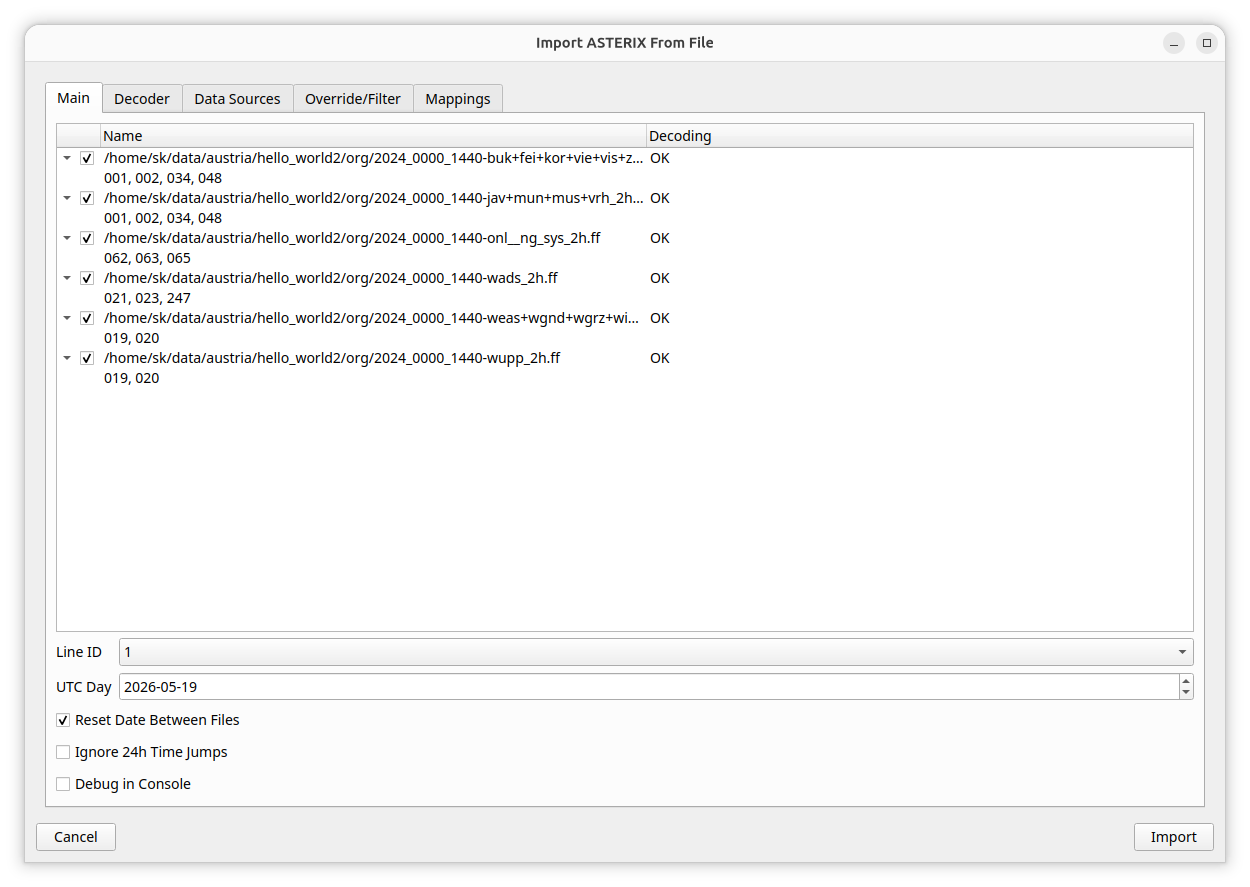
\includegraphics[width=18cm]{figures/asterix_import_data.png}
  \caption{Import ASTERIX data}
\end{figure}

There exist 5 tabs:

\begin{itemize}
\item Main: File label(s) and per-file decoding status, input line
\item Decoder: jASTERIX decoder settings
\item Override / Filter: Data override settings
\item Data Sources: Decode probing results listing data sources and ASTERIX contents
\item Mappings: Definition of created database content based on decoded data
\end{itemize}
\ \\

Please \textbf{note} that the 'Data Sources' tab carries a hint icon when probing reports any warnings, e.g. when a Radar data source has no position configured, when sensors are detected that are not yet present in the active Data Context, or when records lack a usable SAC/SIC. \\

Please \textbf{note} that one or several files can be selected. Since all of the settings are general configuration, please only import several files if they can be imported with the same settings, and do separate imports for non-matching files. \\

The following framings are currently supported:

\begin{itemize}
\item Raw/Netto: Unframed ASTERIX data blocks
\item IOSS: IOSS Final Format
\item IOSS\_SEQ: IOSS Final Format with sequence numbers
\item RFF: Comsoft RFF format
\end{itemize}
\ \\

Please \textbf{note} that the following ASTERIX categories, editions, reserved expansion fields and special purpose fields are currently supported: \\

\begin{tabular}{ | l | r | r | r | r |}
\hline
  CAT & Editions & REFs & SPFs & Used  \\ \hline
  001 & 1.1 & & & X \\ \hline
  002 & 1.0 & & & X  \\ \hline
  004 & 1.4 & & & X  \\ \hline
  010 & 0.24 Sensis, 0.31  &  & & X  \\ \hline
  019 & 1.2, 1.3 & & & X \\ \hline
  020 & 1.5, 1.8 & 1.3 & & X \\ \hline
  021 & 0.26, 2.1, 2.4 & 1.5 & & X \\ \hline
  023 & 1.2 & & & X \\ \hline
  030 & 7.0 & & & \\ \hline
  034 & 1.26 & & &  \\ \hline
  048 & 1.15, 1.23 & 1.9 & & X \\ \hline
  062 & 1.12, 1.16, 1.18, 1.21 & 1.2, 1.4 & ARTAS TRIs & X \\ \hline
  063 & 1.0, 1.1 & & & X \\ \hline
  065 & 1.2, 1.3 & & & X \\ \hline
  247 & 1.2 & & & \\ \hline
  252 & 7.0 & & & \\ \hline
\end{tabular} \\
\  \\

Please \textbf{note} that only the categories marked with 'X' are used, i.e. inserted into the database. Decoding of ASTERIX CAT002 is recommended if CAT001 data is imported, since the timestamps are derived from it (if not available in CAT001).

\subsubsection{Probing}
\label{sec:ui_import_asterix_probing}

Once recording files have been selected, the dialog performs an automatic probing pass that decodes the files in test mode and aggregates the result without writing anything to the database. Probing is re-run whenever the framing, the per-category enable check boxes or the edition / REF / SPF selectors are changed. During probing, a 'Testing Decoding' progress dialog is shown. \\

The probing pass feeds two parts of the import dialog:

\begin{itemize}
\item The file tree on the 'Main' tab, which reports per-file decoding status and per-category record counts
\item The 'Data Sources' tab, which aggregates the probed records per data source and ASTERIX category and joins them with the active Data Context (see \nameref{sec:ui_import_asterix_data_sources_tab})
\end{itemize}
\ \\

The result is read-only; the user proceeds with the import as before. \\

\subsubsection{Main Tab}

At the top, the recording files to be imported are shown in a tree. The tree has the following columns:

\begin{itemize}
\item Checkbox: Indicates whether the file (or section) should be imported
\item Name: Path and filename; for PCAP / network recordings, child rows show the contained sections
\item Decoding: Per-file decoding status from probing
\end{itemize}
\ \\

The 'Decoding' column reports one of the following status values:

\begin{itemize}
\item '?': Not yet tested
\item 'OK': File decoded successfully
\item 'Warning': Decoding succeeded with warnings; the warning text is appended after the colon
\item 'Error': Decoding failed; the error text is appended after the colon
\end{itemize}
\ \\

Hovering the 'Name' column shows a tooltip with the per-category record counts found in the file (e.g. 'CAT001: 12345', 'CAT048: 67890') as well as a 'Total: <N> records' line. \\

Below, the following items exist:
\begin{itemize}
\item Line ID: Line into which all data should be written
\item UTC Day: Date of the recording (for all data)
\item Reset Date Between Files: Use to import non-consecutive files with 24h time jumps (see \nameref{sec:ui_import_asterix_timestamps})
\item Ignore 24h Time Jumps: Do not detect 24h time jumps in input data - import everything into same date (see \nameref{sec:ui_import_asterix_timestamps})
\item Debug in Console: Additional debugging information is output to the console, and the ASTERIX decoding is switched to single-threading for easier investigation
\end{itemize}
\ \\

\subsubsection{Timestamp Calculation}
\label{sec:ui_import_asterix_timestamps}

ASTERIX information does not include useful date information, only \textbf{T}ime \textbf{o}f \textbf{D}ay (\textbf{ToD}), which represents seconds since midnight UTC. The full timestamp is therefore derived from the configured 'UTC Day' plus the ToD, with an automatic 24h rollover detection that advances the day when ToDs near 23:59 reset to values close to 00:00. \\

Since ASTERIX ToDs do not always appear strictly sequentially, the detection allows for a small vicinity around the 24h boundary and only triggers once both late and early values are observed within that window. The vicinity is 5 minutes, i.e. a time jump is set as soon as a ToD of 23:55:00 or later is followed by a ToD of 00:05:00 or earlier. Inside the vicinity, late ToDs keep the previous date and early ToDs get the new date, therefore records which are not in time order are still dated correctly. The detection state is cleared once the ToDs are more than 10 minutes away from midnight. \\

Three controls in the Main tab influence the timestamp calculation:

\begin{itemize}
\item UTC Day: Date given to the first ToD of the import
\item Reset Date Between Files: At each file change, the date is set back to 'UTC Day' and the detection state is cleared. Use it if the next file starts again at its own ToD, instead of continuing the time line of the previous file
\item Ignore 24h Time Jumps: Disables the rollover detection, all ToDs are mapped to the current date
\end{itemize}
\ \\


\includegraphics[width=0.5cm]{../../data/icons/hint.png} Please \textbf{note} that 'Reset Date Between Files' is enabled by default, and that 'Ignore 24h Time Jumps' is disabled by default. \\

\paragraph{Overview}

Two questions define the required settings:

\begin{itemize}
\item Do the selected files continue one time line? Then 'Reset Date Between Files' has to be disabled. Does each file start again at its own ToD? Then it has to be enabled. If only one file is imported, the setting is irrelevant
\item Is a date change in the data real? Then 'Ignore 24h Time Jumps' has to be disabled. Should all data be imported into the same date? Then it has to be enabled
\end{itemize}
\ \\

The following table lists the common recording layouts. Each one is described in the referenced example.

\begin{tabularx}{\textwidth}{ | l | X | l | c | c |}
\hline
  Example & Recording layout & UTC Day & Reset Date & Ignore Jumps \\ \hline
  A & One file, inside one day & Recording day & - & - \\ \hline
  B & One file, across midnight & First day & - & off \\ \hline
  C & Two files, same day, each starting again & Recording day & on & off \\ \hline
  D & Two files, day change at the file cut & First day & \textbf{off} & off \\ \hline
  E & One 24h file, plus minutes of the adjacent days & Main day & - & \textbf{on} \\ \hline
  F & Several files of one day, ToDs near midnight & Recording day & on & \textbf{on} \\ \hline
\end{tabularx} \\
\  \\

A '-' means that the setting has no effect for this layout, therefore it can be left at its default value. 'Reset Date Between Files' has no effect if only one file is imported, since there is no file change. 'Ignore 24h Time Jumps' has no effect if no ToD comes close to midnight. \\

Please \textbf{note} that Example E also requires a Time of Day filter, which is set in the Override / Filter tab (see \nameref{sec:task_import_asterix_override}). \\

\paragraph{Example A: One File Inside One Day}

\begin{figure}[H]
    \centering
    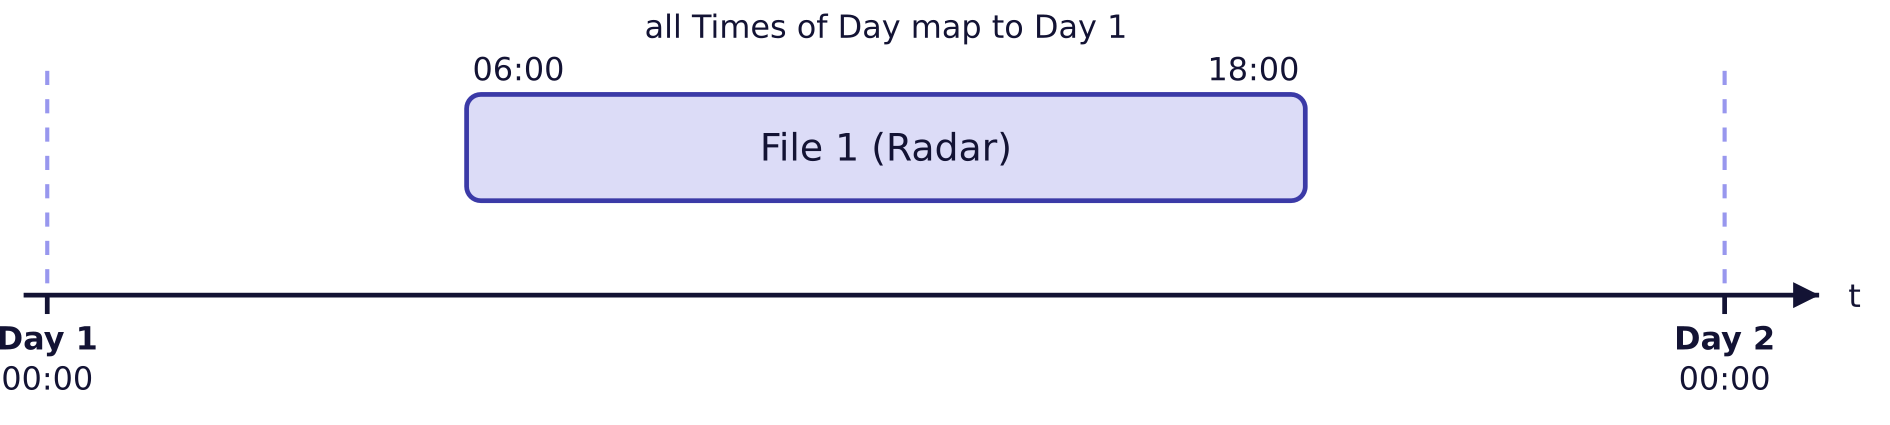
\includegraphics[width=15cm]{figures/asterix_import_ts_a.png}
  \caption{Example A - one file inside one day}
\end{figure}

One recording file which starts and ends inside the same day, e.g. a Radar recording from 06:00 to 18:00. All ToDs are mapped to the recording day.

\begin{itemize}
\item UTC Day: Recording day
\item Reset Date Between Files: No effect, since only one file is imported
\item Ignore 24h Time Jumps: No effect, since no ToD comes close to midnight
\end{itemize}
\ \\

\paragraph{Example B: One File Across Midnight}

\begin{figure}[H]
    \centering
    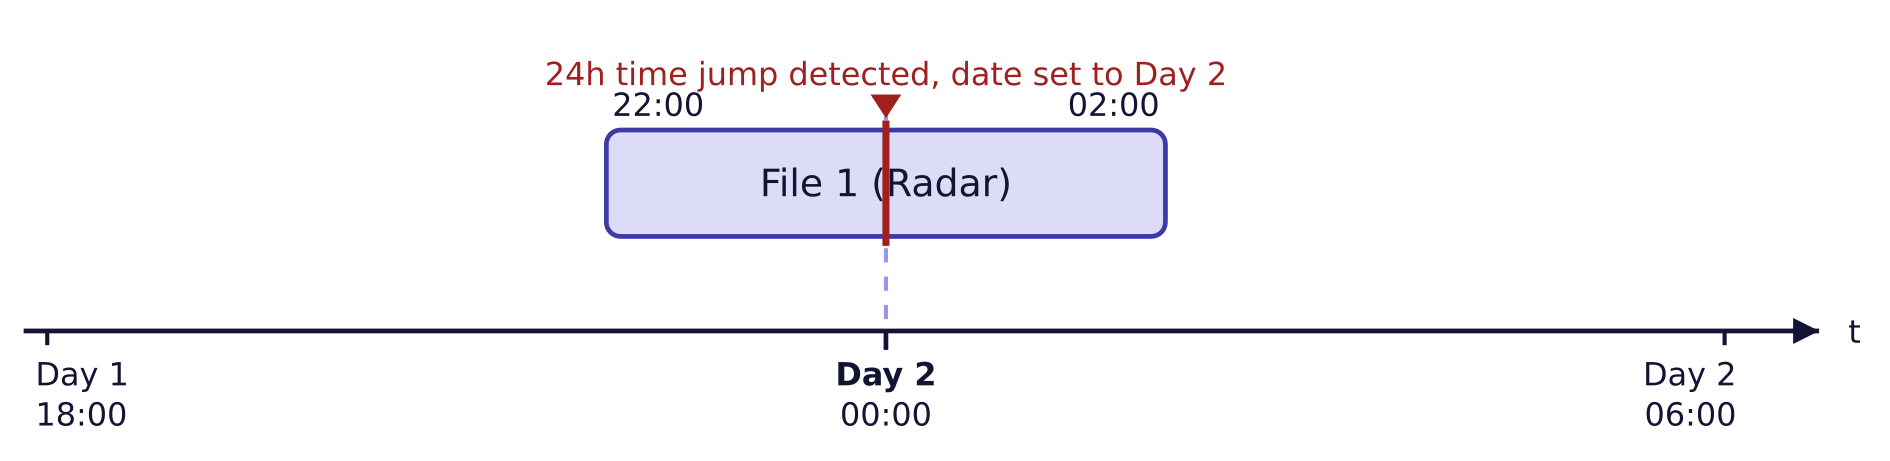
\includegraphics[width=15cm]{figures/asterix_import_ts_b.png}
  \caption{Example B - one file across midnight}
\end{figure}

One recording file which starts before and ends after midnight, e.g. from 22:00 to 02:00. The ToD reset happens inside the file and is detected automatically, therefore all data after midnight gets the next day.

\begin{itemize}
\item UTC Day: First day
\item Reset Date Between Files: No effect, since only one file is imported
\item Ignore 24h Time Jumps: Disabled, which is the default. If it is enabled, the data after midnight is dated one day too early
\end{itemize}
\ \\

\paragraph{Example C: Two Files of the Same Day}

\begin{figure}[H]
    \centering
    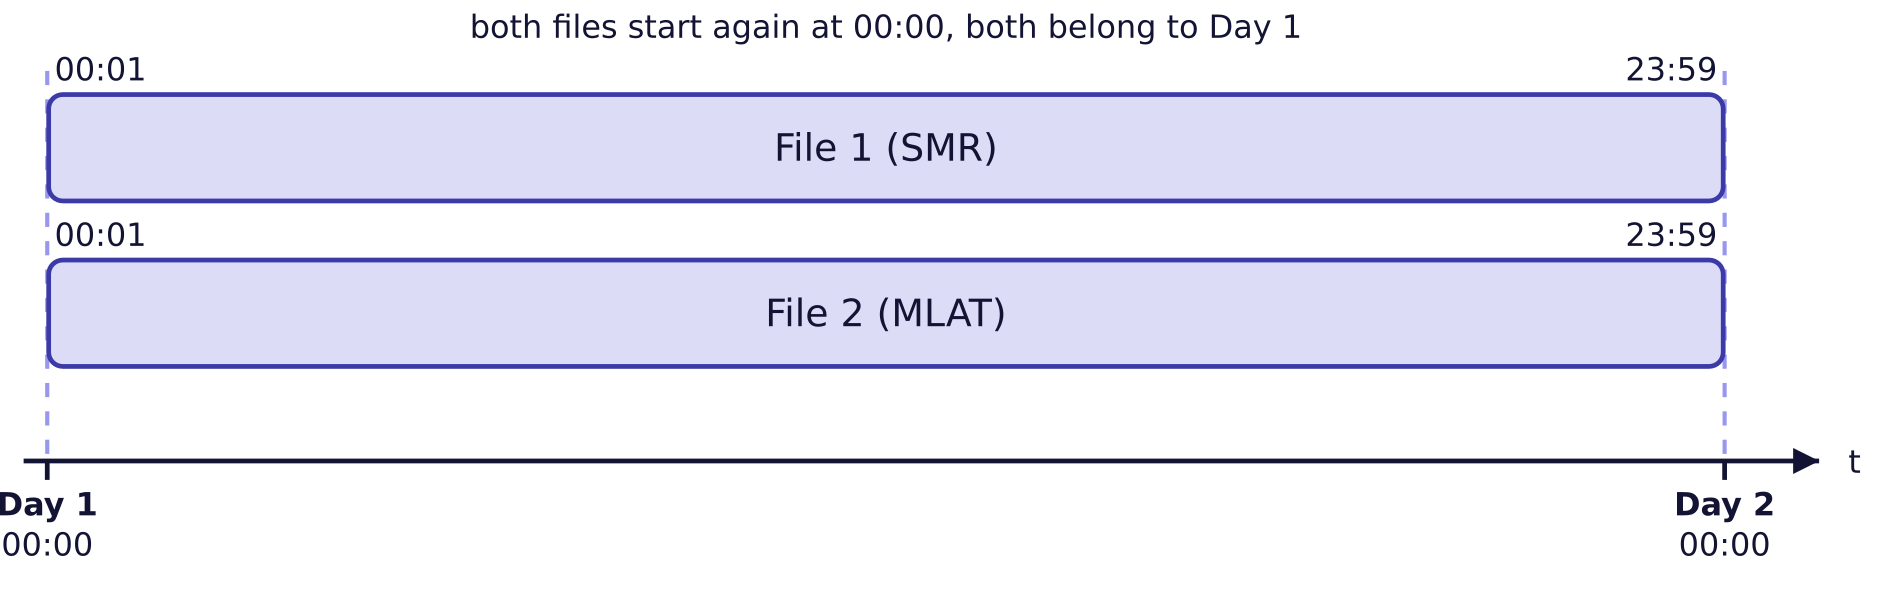
\includegraphics[width=15cm]{figures/asterix_import_ts_c.png}
  \caption{Example C - two files of the same day}
\end{figure}

Two files which cover the same day, e.g. one SMR file and one MLAT file, both from 00:01 to 23:59. Each file starts again at its own ToD.

\begin{itemize}
\item UTC Day: Recording day
\item Reset Date Between Files: Enabled, which is the default. If it is disabled, the late ToDs at the end of the first file and the early ToDs at the start of the second file are read as a 24h time jump, and the second file is dated one day too late
\item Ignore 24h Time Jumps: Disabled, which is the default. A time jump inside one of the files is then still detected
\end{itemize}
\ \\

\paragraph{Example D: Two Files With the Day Change at the File Cut}

\begin{figure}[H]
    \centering
    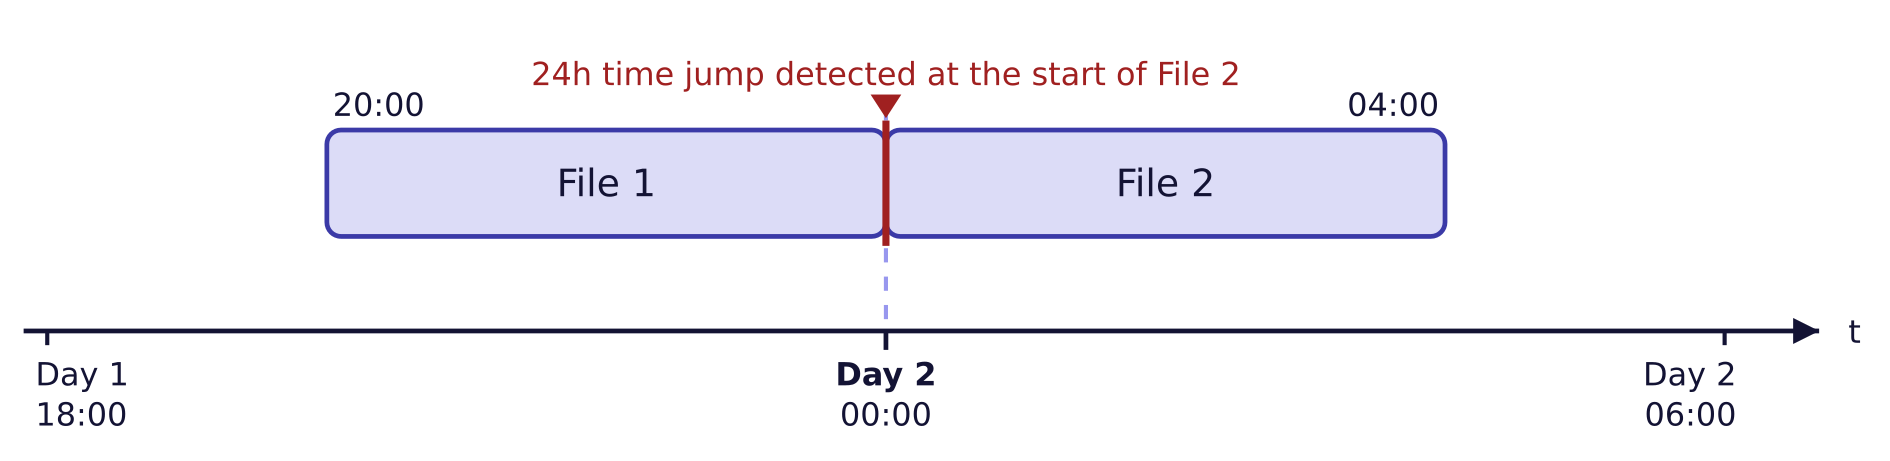
\includegraphics[width=15cm]{figures/asterix_import_ts_d.png}
  \caption{Example D - two files with the day change at the file cut}
\end{figure}

Two files which continue one time line, where the day changes at the cut between them, e.g. file 1 from 20:00 to 24:00 and file 2 from 00:00 to 04:00.

\begin{itemize}
\item UTC Day: First day
\item Reset Date Between Files: \textbf{Disabled}, which is not the default. The late ToDs of file 1 and the early ToDs of file 2 are then used together, and the time jump is detected at the start of file 2. If it is enabled, file 2 is set back to 'UTC Day', and all of its data is dated one day too early
\item Ignore 24h Time Jumps: Disabled, which is the default. The time jump at the file cut must be detected
\end{itemize}
\ \\

Please \textbf{note} that the files are decoded in the order in which they are listed in the Main tab. \\

\paragraph{Example E: One 24h File With Data of the Adjacent Days}

\begin{figure}[H]
    \centering
    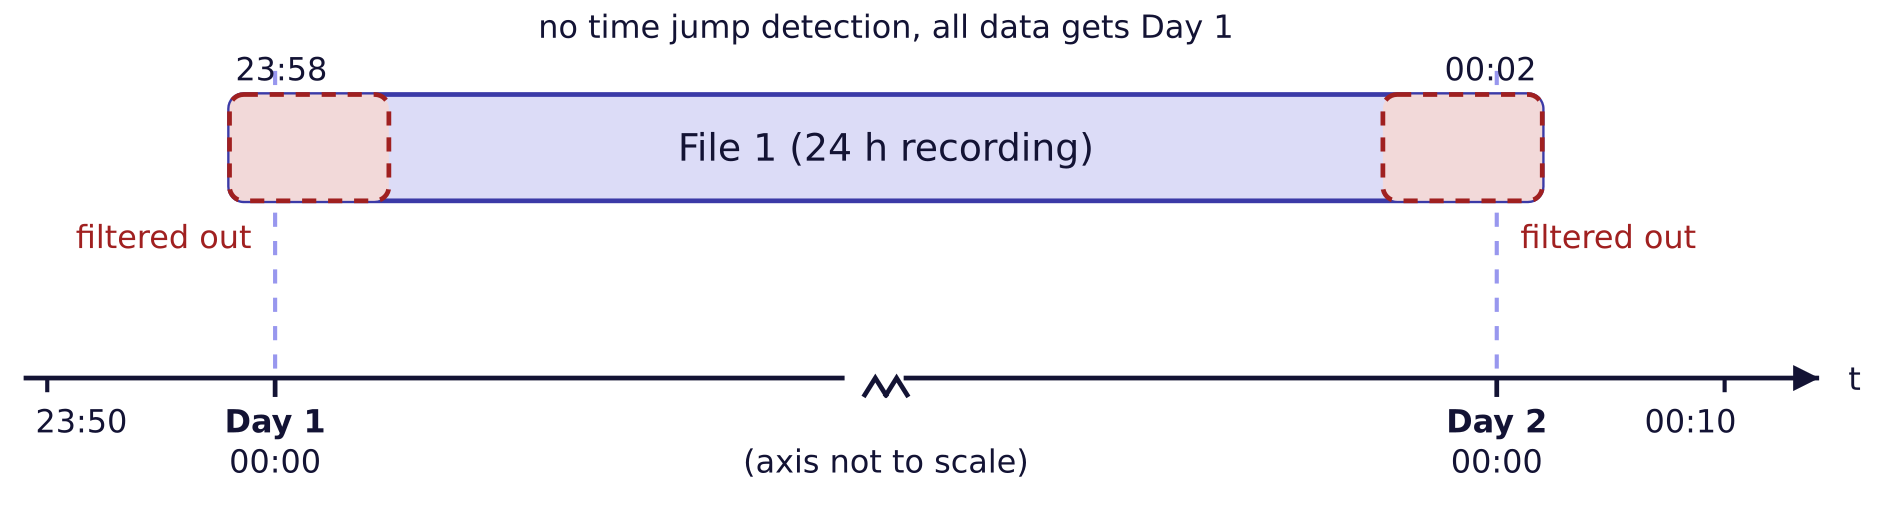
\includegraphics[width=15cm]{figures/asterix_import_ts_e.png}
  \caption{Example E - one 24h file with data of the adjacent days}
\end{figure}

One recording file which covers one full day, but also holds a few minutes of the previous and of the next day, e.g. from 23:58 to 00:02. All data is dated with the main day, and the minutes of the adjacent days are removed by a filter.

\begin{itemize}
\item UTC Day: Main day
\item Reset Date Between Files: No effect, since only one file is imported
\item Ignore 24h Time Jumps: \textbf{Enabled}, which is not the default. If it is disabled, the minutes of the previous day at the start of the file are read as a 24h time jump, and the whole main day is dated one day too late
\item Filter Time of Day: Enabled, with the range 00:05:00 to 23:55:00, set in the Override / Filter tab (see \nameref{sec:task_import_asterix_override}). The minutes of the adjacent days are imported with a wrong date, and are removed by this filter
\end{itemize}
\ \\


\includegraphics[width=0.5cm]{../../data/icons/hint.png} Please \textbf{note} that the Time of Day filter is applied after the timestamp calculation. It can therefore not prevent a wrong 24h time jump. It also removes the first and the last minutes of the wanted day, since the filter works on the ToD only. \\

\paragraph{Example F: Several Files of One Day}

\begin{figure}[H]
    \centering
    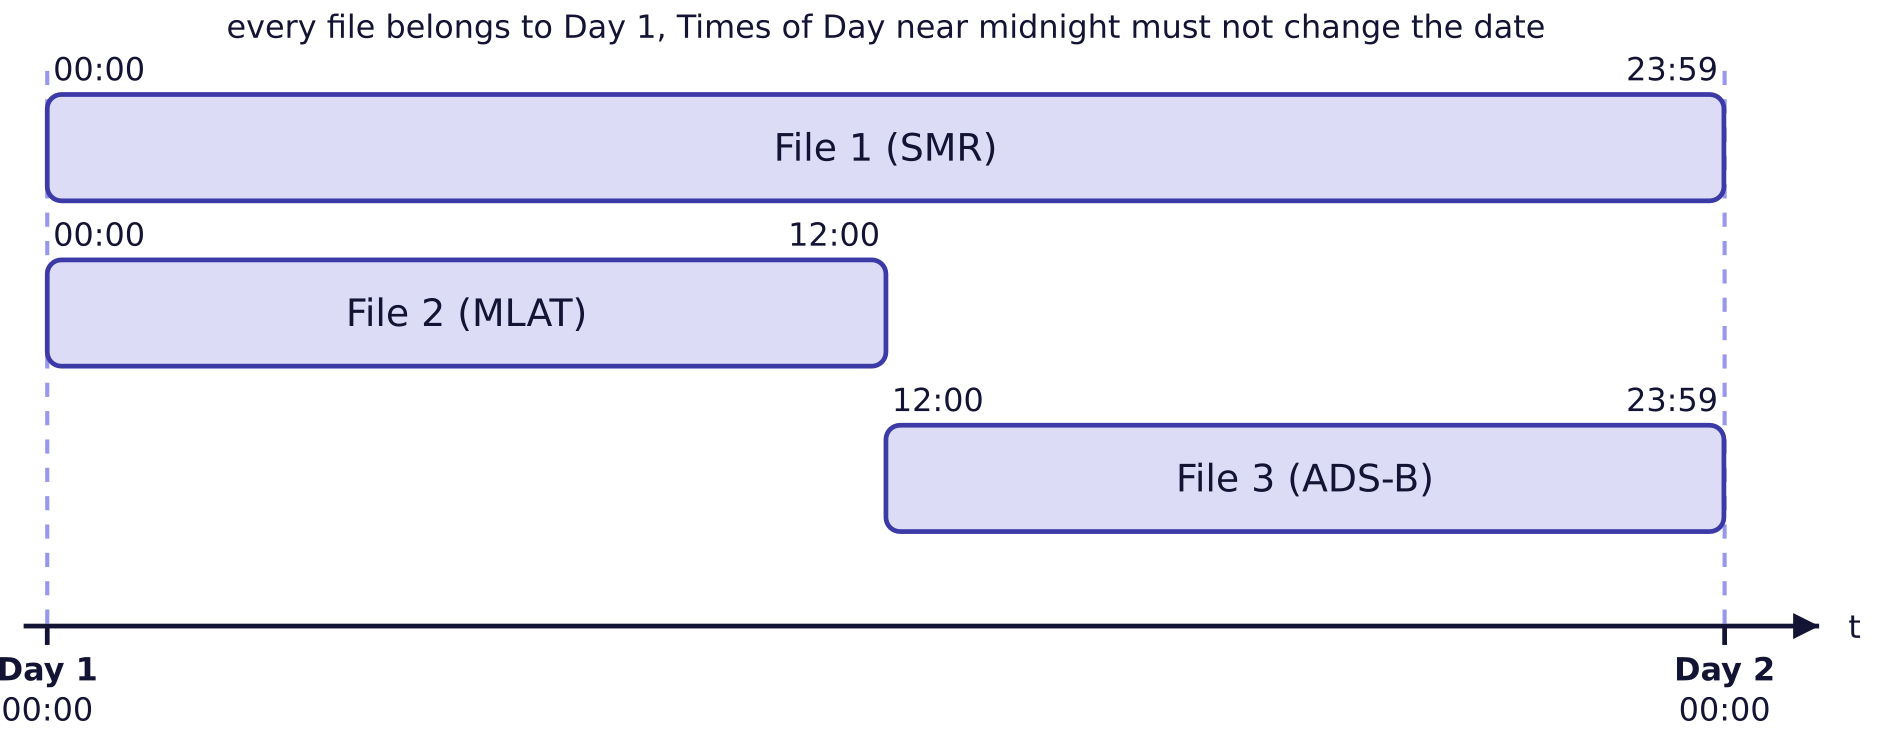
\includegraphics[width=15cm]{figures/asterix_import_ts_f.png}
  \caption{Example F - several files of one day}
\end{figure}

Several files which all belong to one day, e.g. one file per sensor, not necessarily covering the same hours. Every ToD is mapped to 'UTC Day'.

\begin{itemize}
\item UTC Day: Recording day
\item Reset Date Between Files: Enabled, which is the default. Each file starts again at its own ToD
\item Ignore 24h Time Jumps: \textbf{Enabled}, which is not the default. Use it if the files hold records close to midnight, e.g. a few records of the previous or of the next day, or records which are not in time order there. No date change can then happen
\end{itemize}
\ \\

Please \textbf{note} that a real date change is no longer detected with this setting. It must therefore only be used for data of one day. \\

\paragraph{Cases Which Require Several Imports}

All settings are applied to all selected files. The following cases can therefore not be handled in one import, and require one import per group of files:

\begin{itemize}
\item Recordings of different days: Only one 'UTC Day' exists per import. Import each day separately, with the matching 'UTC Day'
\item Data for different lines: Only one 'Line ID' exists per import. Import each line separately, e.g. a first recording into L1 and a second recording of the same sensors into L2
\item Files which require different settings of the two check boxes, e.g. a continuous pair of files together with a separate single file
\item Files which require different Override / Filter settings, e.g. a different Time of Day offset per file
\end{itemize}
\ \\

\paragraph{Checking the Result}

After the import, the resulting dates should be checked:

\begin{itemize}
\item The 'Timestamps' 'Min' and 'Max' values at the bottom of the Data Sources tool show the time span of all data in the database (see \nameref{sec:data_sources}). Both dates and times must match the expected recording period
\item The Task Log lists one message per detected 24h time jump, as well as the last ToD and timestamp of each decoded file (see \nameref{sec:task_log})
\end{itemize}
\ \\

Please \textbf{note} that a wrong date commonly shows as a time span of about 2 days instead of 1, or as a gap of exactly 24 hours between the data of different sensors. In such a case the data should be imported again with corrected settings.


\subsubsection{Decoder}

In this tab, all decoder settings can be configured. Please \textbf{note} that changing the settings will trigger a re-evaluation if the recordings can be imported correctly, 
therefore changing the information displayed in the main tab.

\begin{figure}[H]
    \centering
    \hspace*{-1.5cm}
    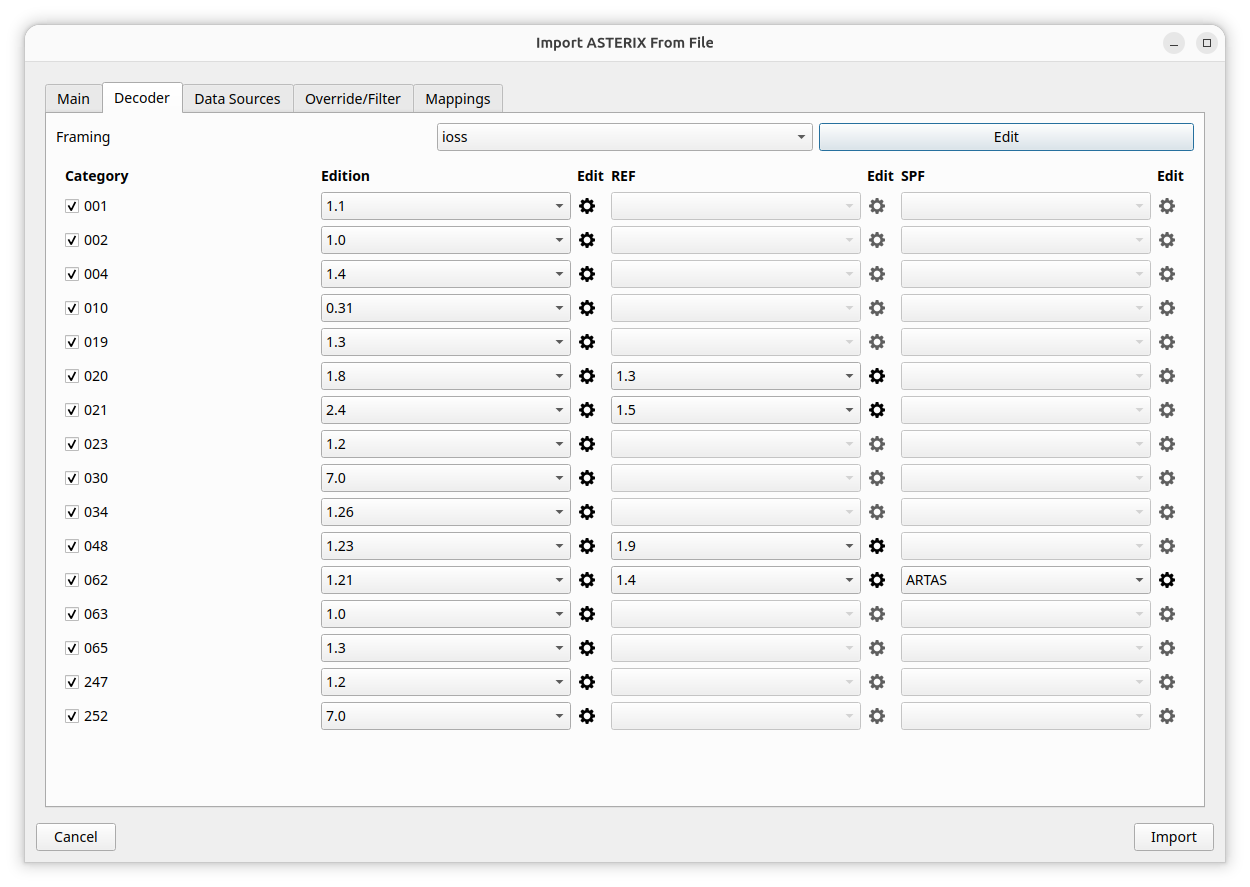
\includegraphics[width=18cm]{figures/asterix_import_data_decoder.png}
  \caption{Import ASTERIX data Decoder}
\end{figure}

\paragraph{Framing}
Using the 'Framing' drop-down menu, the current framing can be selected. Using the 'Edit' button, the current framing definition is opened in a text editor.

\paragraph{Categories}

For each category, a number of elements exist:

\begin{itemize}
\item Category checkbox: Number of category and checkbox defining if it should be decoded
\item Edition: Drop-down menu to select the edition number to be used
\item Edition Edit Button \includegraphics[width=0.5cm]{../../data/icons/edit.png}: Opens the current edition definition in a text editor
\item REF: Drop-down menu to select the Reserved Expansion Field definition (if available)
\item REF Edit Button \includegraphics[width=0.5cm]{../../data/icons/edit.png}: Opens the current REF definition in a text editor
\item SPF: Drop-down menu to select the Special Purpose Field definition (if available)
\item SPF Edit Button \includegraphics[width=0.5cm]{../../data/icons/edit.png}: Opens the current SPF definition in a text editor
\end{itemize}
\ \\

\paragraph{Additional}

Using the 'Edit Data Block' button, the ASTERIX data block definition is opened in a text editor. \\

Using the 'Edit Categories' button, the ASTERIX definitions file is opened in a text editor. \\

Using the 'Refresh' button, all of the jASTERIX definitions are reloaded from the hard disk (e.g. to update after file changes were made). \\

\subsubsection{Data Sources Tab}
\label{sec:ui_import_asterix_data_sources_tab}

This tab aggregates the probing pass per data source and per ASTERIX category, and joins the result with the data sources defined in the active Data Context. The tab is split into a tree on the left and a detail area on the right. \\

\begin{figure}[H]
    \centering
    \hspace*{-1.5cm}
    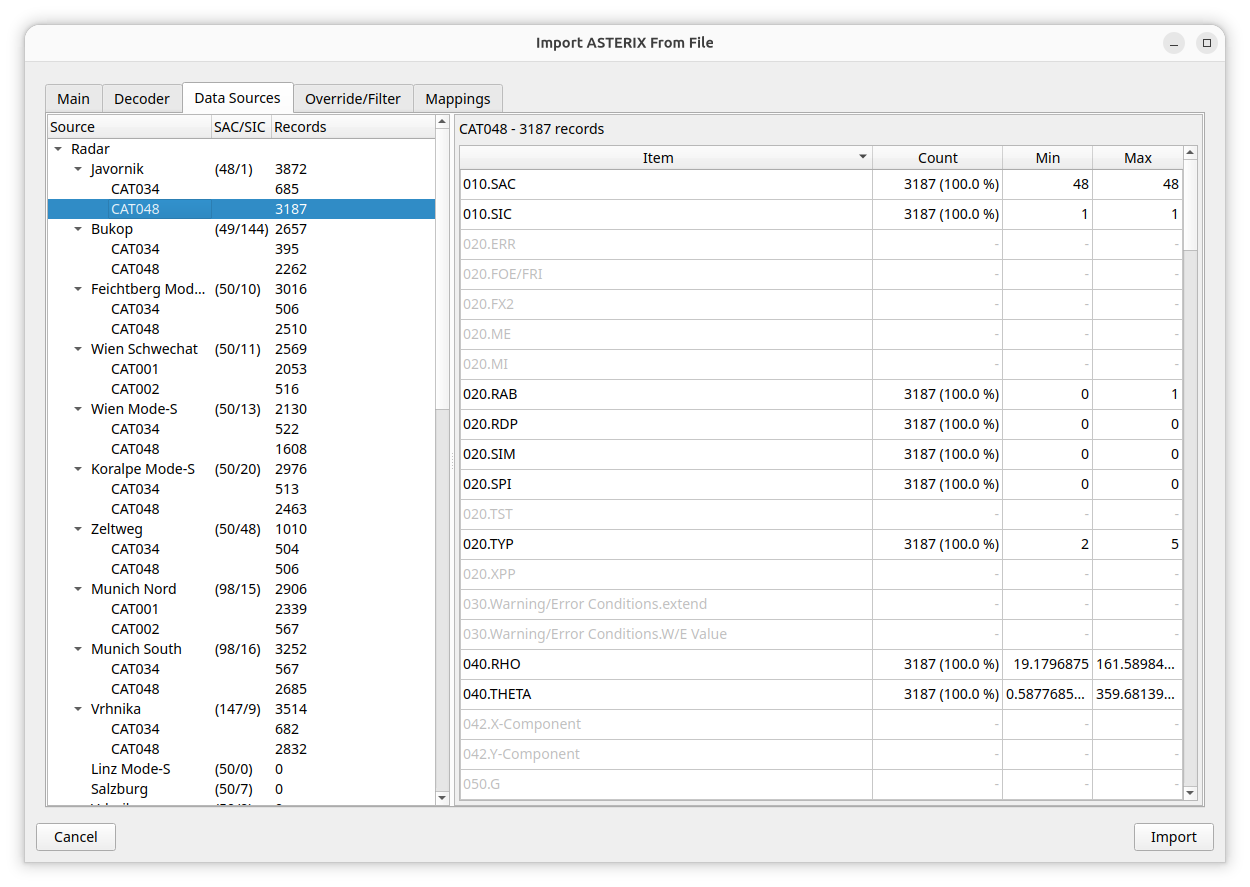
\includegraphics[width=18cm]{figures/asterix_import_data_sources.png}
  \caption{ASTERIX Import: Data Sources tab}
\end{figure}

The tab applies to file imports only. Until the probing pass has produced data, the detail area shows a placeholder text:

\begin{itemize}
\item 'Data Sources tab applies to file imports only.': The current import source is a network feed
\item 'Run the decoding check to populate data source information.': Probing has not yet produced any results
\item 'Select a data source or category to see details.': Normal state, no tree row selected
\end{itemize}
\ \\

\paragraph{Tree}

The tree has 3 columns: 'Source', 'SAC/SIC' and 'Records'. Top-level entries are DSType groups (Radar, MLAT, ADS-B, Tracker, RefTraj, Other) in canonical order. Each group lists its data sources, each data source lists the ASTERIX categories observed during probing. \\

\begin{itemize}
\item DSType group row: Name of the DSType. Carries a hint icon when one of its data sources has a warning.
\item Data source row: Source name (or 'DS ID' if unnamed), SAC/SIC and the total record count across all categories. A hint icon is shown when a warning applies (e.g. a Radar without configured position, an 'Other' DSType, or a probe-only data source).
\item Category row: 'CATXXX' in the 'Source' column and the per-category record count in the 'Records' column.
\end{itemize}
\ \\

Two special top-level groups may appear:

\begin{itemize}
\item 'Detected (not in context)': Sensors that were found in the probed data but are not yet defined in the active Data Context. The group carries the tooltip 'These sensors were detected in the probed data but are not yet defined in the active context.'. Each child row is labeled 'Unknown sensor' and shows the probed SAC/SIC.
\item 'Unknown SAC/SIC': Aggregates records that lack a usable SAC/SIC (typically CAT001 / CAT002 records with a missing I010 item).
\end{itemize}
\ \\

\paragraph{Data Source Detail}

Selecting a data source row in the tree shows the data source detail widget on the right, identical to the one used in the Data Context dialog (see \nameref{sec:ui_configure_data_sources}). \\

If the selected entry is a probe-only data source (detected but not in the context), a banner is shown above the editor with the text 'This sensor was detected in the probed data but is not yet in the active context.', along with an 'Add to Context' button (tooltip 'Create this data source in the active context using the values entered below.'). Confirming the button creates the data source in the active Data Context using the values currently entered in the editor. \\

\paragraph{Category Detail}

Selecting a 'CATXXX' row shows the per-item statistics table on the right, with a header label of the form 'CATXXX - <count> records' (or 'CATXXX - no records' when no record was observed). \\

The table has the following columns:

\begin{itemize}
\item Item: Dotted ASTERIX data item name (e.g. '010', '050', '070.Mode3A')
\item Count: Number of probed records carrying the item, followed by the percentage relative to the category total (e.g. '1234 (99.7\%)'); '-' if the item was not seen
\item Min: Minimum value observed during probing, or '-' if not seen
\item Max: Maximum value observed during probing, or '-' if not seen
\end{itemize}
\ \\

Items that are defined in the selected jASTERIX edition but were not observed during probing are listed in disabled text color. The table can be sorted by clicking the column headers. \\


\subsubsection{Override / Filter Tab}
\label{sec:task_import_asterix_override}

\begin{figure}[H]
  \centering
    \hspace*{-1.5cm}
    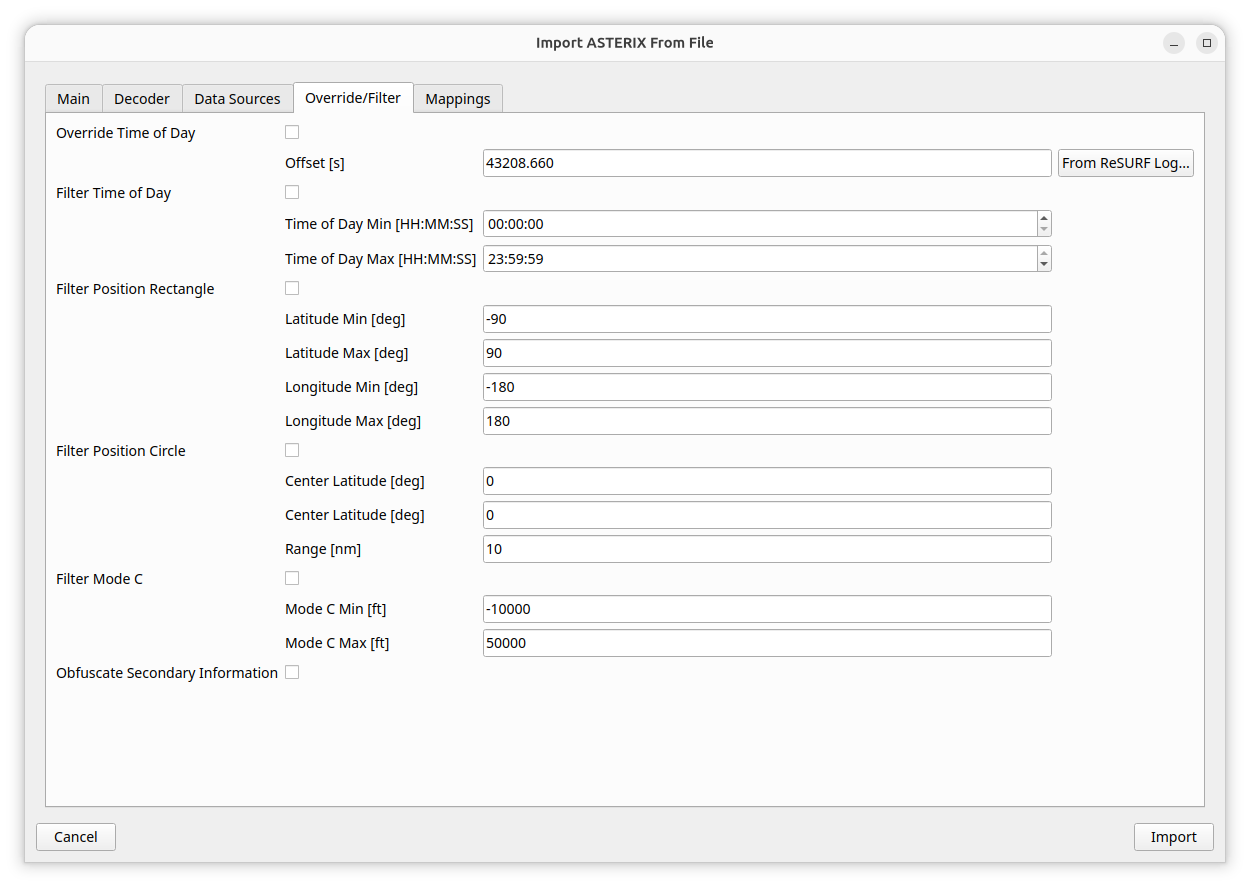
\includegraphics[width=18cm]{figures/asterix_import_data_override.png}
  \caption{ASTERIX Import Data Override / Filter}
\end{figure}

These features should only be used in very specific circumstances.

\begin{itemize}
\item Time Correction
\begin{itemize}
\item Override Time of Day: Checkbox enabling the Time of Day offset to be added, to correct for unwanted time-shifts
\item Offset [s]: Positive or negative offset to be added, in seconds. Range -86400 to +86400 with up to 5 decimals. If the resulting value is out of bounds, it is adjusted to the [0, 86400] interval.
\item From ReSURF Log...: Calculates the offset from ReSURF log output. Opens a paste dialog that accepts lines of the form

\begin{lstlisting}
File input=...: first frame time set to HH:MM:SS.ss
File input=...: rendez-vous time set to HH:MM:SS.ss
\end{lstlisting}

and auto-fills the offset accordingly.
\end{itemize}
\item Filters
\begin{itemize}
\item Filter Time of Day: Use minimum / maximum times, everything outside will be ignored
\item Filter Position Rectangle: Use minimum / maximum rectangle in latitude and longitude
\item Filter Position Circle: Use center position latitude and longitude and range in nautical miles
\item Filter Mode C: Use minimum / maximum rectangle in Mode C. Target reports without Mode C will not be filtered.
\end{itemize}
\item Obfuscate Secondary Information: Replaces secondary-identification values with deterministic random surrogates - the same input value always maps to the same output within the session
\begin{itemize}
\item Mode 3/A: random 12-bit replacement, except for conspicuity codes (octal 0000, 1000, 2000, 7500, 7600, 7700, 7776, 7777) which pass through unchanged.
\item Mode S Aircraft Address (ACAD): random 24-bit ICAO address (range 1 to 0xFFFFFF)
\item Mode S Aircraft Identification (ACID): replaced with a starship-name-derived string of the same letter length
\end{itemize}
\end{itemize}
\ \\

Please \textbf{note} that the filtering is applied after the (optional) 'Time of Day' correction is performed. Also, if any filters are active, the import status dialog may not be updated for some time and show wrong time estimates.
\\

Please also \textbf{note} that the obfuscation function currently only overrides the main DBContent variables, i.e. the one used for labels. Other additional secondary values could still be set in the database, therefore this function exists mainly for presentation purposes, not to safeguard against all use cases. Also, to create a time-shift in the data, it is recommended to set a wrong 'UTC Day' as well as to add a random 'Time of Day' override offset.


\subsubsection{Mappings Tab}

\begin{figure}[H]
  \centering
    \hspace*{-1.5cm}
    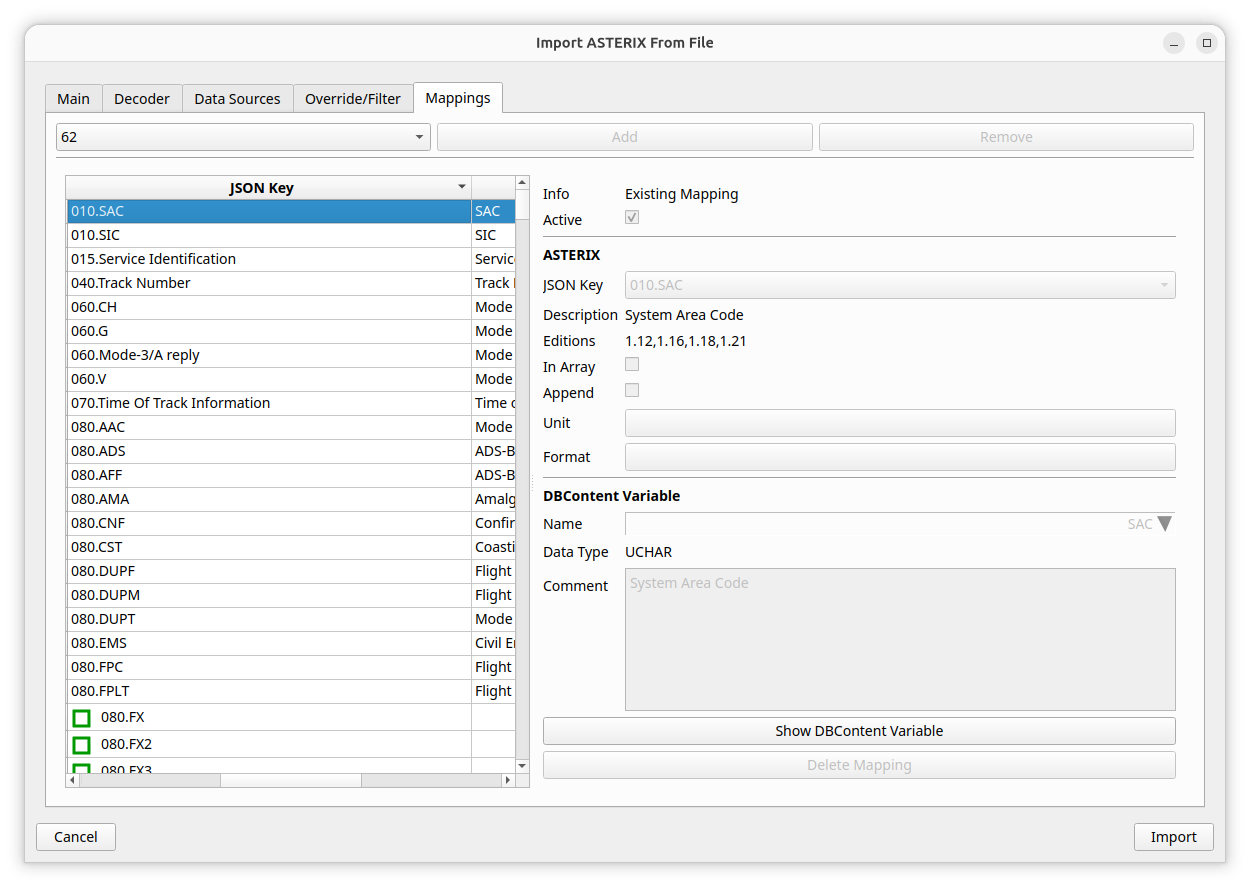
\includegraphics[width=18cm]{figures/asterix_import_data_mappings.png}
  \caption{ASTERIX Import Data Mappings}
\end{figure}

At the top, the GUI elements can be used to show/add/remove ASTERIX JSON parsers. Below, the currently selected ASTERIX JSON parser is shown and can be configured. \\

An ASTERIX JSON parser in this context is the function that parses the JSON content created by the jASTERIX parser, and creates DBContent from it. 
For each ASTERIX category a dedicated parser defines the mapping from JSON to a DBContent. \\

For the common user interaction is normally not recommended, but it can be used to understand what DBContent is created from what ASTERIX data.

\paragraph{Top Elements}

Using the drop-down menu, the parser to be shown can be selected. The buttons allow for adding and removing ASTERIX JSON object parsers.

\paragraph{Parser GUI Elements}

The exact definition of how the parsing works is out of scope for this document, so only a short summary is given here. For more information please contact the author.

In the mappings list, the following columns are given:

\begin{itemize}
\item Active checkbox: Defines if the specific mapping is used
\item JSON Key: JSON location and name of the data to be mapped, commonly in 'Data Item Number'.'Variable' or 'Data Item Number'.'Sub Item'.'Variable' format
\item DBContent Variable: Target variable to which this data is mapped
\end{itemize}
\ \\

Whenever a mapping is selected, the details are shown on the right side, providing information about the ASTERIX data item (based on the jASTERIX specifications) and the DBContent variable it is mapped to. 
Using the 'Show DBContent Variable' button the variable can be inspected in detail.

\begin{figure}[H]
  \centering
    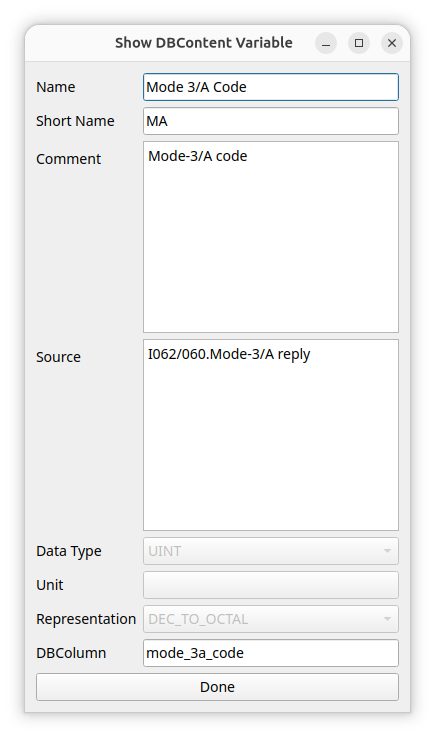
\includegraphics[width=7cm]{figures/asterix_import_data_dbcont_var_details.png}
  \caption{Task: Import ASTERIX Data DBContent Variable Details}
\end{figure}

\subsubsection{Running}

The 'Cancel' button aborts the import.  The 'Import' button triggers the import of the selected files into the database with the given options, but is only available if all selected files can be decoded correctly. \\

Using the 'Import' button, the import task can be performed. During import a status indication will be shown. \\

\begin{figure}[H]
    \centering
    \hspace*{-1.5cm}
    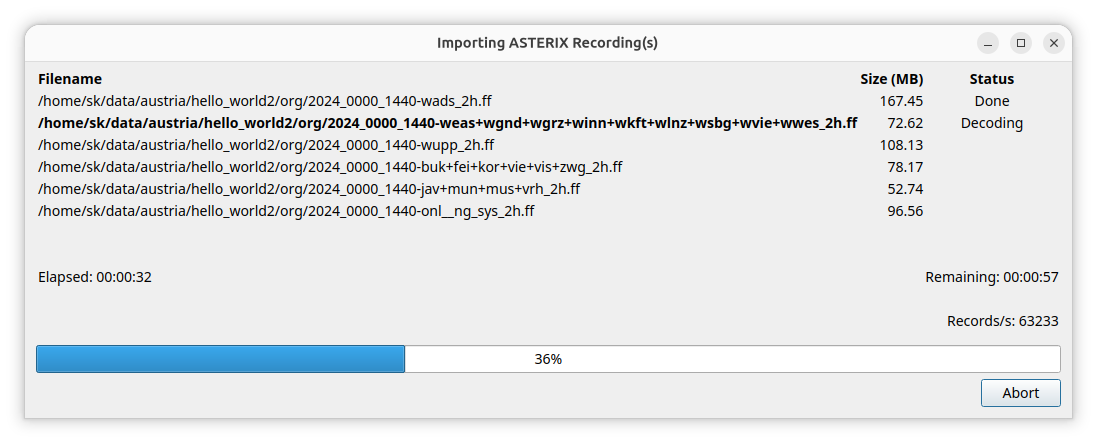
\includegraphics[width=18cm]{figures/asterix_import_data_status.png}
  \caption{Import ASTERIX data status}
\end{figure}

If a decoding error occurs even if the ASTERIX probing did not previously detect any, an error is indicated in the status dialog. Errors encountered during import - failed records, decoding errors and missing definitions - are aggregated into the notes of the import report shown after the run completes, rather than only being written to the log. \\


Please make sure that the correct framing and edition versions are selected, or contact the author for support if this does not resolve the issue. \\

\subsubsection{Report}

After an import run completes, a task report named 'ASTERIX Import' is generated and shown in the Reports tool of the Flight Deck (see \nameref{sec:reports}). The report is appended to across runs: each subsequent ASTERIX import adds new rows and sections rather than overwriting the previous ones. \\

The report is organized as follows:

\begin{itemize}
\item Overview: 'Imported Files' table with one row per imported file, containing the columns '\#', 'Begin', 'Elapsed', 'File', 'Size', 'Source', 'Framing', 'Errors', 'Warnings'. Each row links to the corresponding per-file section.
\item Files: One sub-section per imported file, containing:
  \begin{itemize}
  \item Info: Filename, path, size, content info, source, framing, import timestamp, elapsed time, number of PCAP sections (if any).
  \item Records per Data Source: For each detected data source, the DS Type and the per-DBContent record counts; each row links to the corresponding data source detail sub-section.
  \item One sub-section per DSType, with one sub-section per Data Source, with one table per ASTERIX category. Each table lists the data items observed during probing ('Item', 'Count', 'Min', 'Max', 'Description'); items defined in the active edition but not seen during probing are listed with count 0 and highlighted in red.
  \item Errors / Warnings: Text block listing probe-time errors and warnings of the file and its sections, when present.
  \end{itemize}
\end{itemize}
\ \\

Please \textbf{note} that the per-data-item statistics in the report are derived from the probing pass (see \nameref{sec:ui_import_asterix_probing}), which reads only the beginning of each file. Counts, minima and maxima are therefore sample-side estimates and do not necessarily reflect the full file. Errors encountered during the actual import are aggregated separately into the report's notes. \\

\paragraph{Comments}
The time needed for the import strongly depends on the available CPU performance (multithreading being very beneficial), but an import of 5 million target reports takes about 2 minutes on the author's hardware. \\

The (truncated) timestamps of CAT001 are calculated in a simple algorithm based on the CAT002 messages from the same sensor, so their timestamp data is a bit unreliable, but exact enough for e.g. time window filtering. \\

This task can be run several times, e.g. if multiple ASTERIX recordings from different data sources are to be imported. \\


\includegraphics[width=0.5cm]{../../data/icons/hint.png} Please \textbf{note} that currently not all data fields (as shown in the JSON object parsers) are imported.


